\begin{figure}[htbp]
\centering
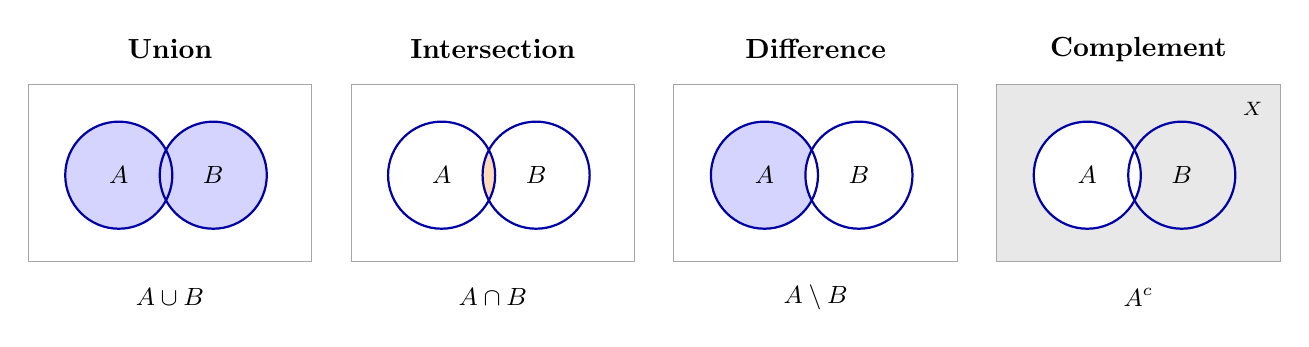
\begin{tikzpicture}[font=\small]
    \foreach \shift/\title in {0/{Union},4.1/{Intersection},8.2/{Difference},12.3/{Complement}} {
        \begin{scope}[xshift=\shift cm]
            \node[font=\bfseries] at (1.8,2.7) {\title};
        \end{scope}
    }
    \begin{scope}
        \fill[blue!17] (1.15,1.1) circle (0.68);
        \fill[blue!17] (2.35,1.1) circle (0.68);
        \draw[gray!70] (0,0) rectangle (3.6,2.25);
        \draw[blue!65!black,thick] (1.15,1.1) circle (0.68);
        \draw[blue!65!black,thick] (2.35,1.1) circle (0.68);
        \node at (1.15,1.1) {$A$};\node at (2.35,1.1) {$B$};
        \node at (1.8,-0.45) {$A\cup B$};
    \end{scope}
    \begin{scope}[xshift=4.1cm]
        \begin{scope}
            \clip (1.15,1.1) circle (0.68);
            \fill[orange!28] (2.35,1.1) circle (0.68);
        \end{scope}
        \draw[gray!70] (0,0) rectangle (3.6,2.25);
        \draw[blue!65!black,thick] (1.15,1.1) circle (0.68);
        \draw[blue!65!black,thick] (2.35,1.1) circle (0.68);
        \node at (1.15,1.1) {$A$};\node at (2.35,1.1) {$B$};
        \node at (1.8,-0.45) {$A\cap B$};
    \end{scope}
    \begin{scope}[xshift=8.2cm]
        \fill[blue!17] (1.15,1.1) circle (0.68);
        \begin{scope}
            \clip (1.15,1.1) circle (0.68);
            \fill[white] (2.35,1.1) circle (0.68);
        \end{scope}
        \draw[gray!70] (0,0) rectangle (3.6,2.25);
        \draw[blue!65!black,thick] (1.15,1.1) circle (0.68);
        \draw[blue!65!black,thick] (2.35,1.1) circle (0.68);
        \node at (1.15,1.1) {$A$};\node at (2.35,1.1) {$B$};
        \node at (1.8,-0.45) {$A\setminus B$};
    \end{scope}
    \begin{scope}[xshift=12.3cm]
        \fill[gray!18] (0,0) rectangle (3.6,2.25);
        \fill[white] (1.15,1.1) circle (0.68);
        \draw[gray!70] (0,0) rectangle (3.6,2.25);
        \draw[blue!65!black,thick] (1.15,1.1) circle (0.68);
        \draw[blue!65!black,thick] (2.35,1.1) circle (0.68);
        \node at (1.15,1.1) {$A$};\node at (2.35,1.1) {$B$};
        \node at (1.8,-0.45) {$A^c$};
        \node[anchor=north east,font=\scriptsize] at (3.5,2.15) {$X$};
    \end{scope}
\end{tikzpicture}
\caption{Venn diagrams for union, intersection, relative difference, and complement in the fixed universe $X$; the shaded area is the set named below each panel.}
\label{fig:set-operations-venn}
\end{figure}